% chapters/seismo.tex
%
% Copyright 2022 Alexander Lyttle.
%
% This work may be distributed and/or modified under the conditions of the
% LaTeX Project Public License (LPPL) version 1.3 or later.
%
% The latest version of this license is in
% https://www.latex-project.org/lppl.txt and version 1.3 or later is part of
% all distributions of LaTeX version 2005/12/01 or later.
%
%
\chapter[Asteroseismology]{Asteroseismology of Solar-Like Oscillators}

Several decades ago, 5-minute oscillations of solar surface radial velocity were observed by \citet{Leighton.Noyes.ea1962}, leading to the inference of acoustic waves trapped beneath the solar photosphere \citep{Ulrich1970}. A further decade of study culminated in the measurement of individual oscillation modes in the Doppler radial velocity \citep{Claverie.Isaak.ea1979} and total irradiance \citep{Woodard.Hudson1983a} of the Sun. Initially thought to be short-lived irregularities on the surface, these modes were found to be compatible with stochastically excited standing waves penetrating deep into the Sun. Later, \citet{Deubner.Gough1984} introduced the word \emph{helioseismology} (analogous to geo-seismology) to describe the study of the solar interior using observations of these modes. Helioseismology was soon responsible for breakthrough solar research, from measuring differential rotation \citep{Deubner.Ulrich.ea1979} to solving the mismatch between predicted and measured solar neutrino production \citep{Bahcall.Ulrich1988}.

Astronomers initially debated the mechanism driving solar oscillations in the form of standing pressure waves (or \emph{p modes}). \citet{Goldreich.Keeley1977} suggested what became the prevailing theory, that the p modes were stochastically excited by near-surface convection. Hence, we might expect solar-like oscillations to be present in other stars which have a convective envelope similar to the Sun. Shortly thereafter, \citet{Christensen-Dalsgaard1984} introduced the term \emph{asteroseismology} --- the study of the internal structure of stars with many observable modes of oscillation. Subsequently, solar-like oscillations were discovered in a few bright stars. Among the first were Procyon and \(\alpha\) Cen A \citep{Gelly.Grec.ea1986}, with individual modes later resolved by \citet{Martic.Schmitt.ea1999} and \citet{Bouchy.Carrier2001} respectively.

Instrumental and atmospheric noise limited the progress of asteroseismology with ground-based equipment to studies of small number of bright dwarf stars. Asteroseismology requires high-cadence (\(\sim \SIrange{1}{10}{\minute}\)) brightness observations over long time-periods (\(\sim \SI{1}{\year}\)) with precisions of \todo{precision}. The first dedicated space-based missions which met these requirements arrived in the late 2000s, accelerating progress in the field. Initially, \emph{CoRoT} \citep{Baglin.Auvergne.ea2006} detected solar-like oscillations in thousands of red giant stars \citep{DeRidder.Barban.ea2009,Mosser.Belkacem.ea2010}. Then, \emph{Kepler} \citep{Borucki.Koch.ea2010} found oscillations in thousands more red giants \citep{Pinsonneault.Elsworth.ea2014} and hundreds of main sequence stars similar to the Sun \citep{Serenelli.Johnson.ea2017}. Most recently, \emph{TESS} \citep{Ricker.Winn.ea2015} has added thousands more dwarf and giant stars to the roster of solar-like oscillators \citep{Hon.Huber.ea2021,SilvaAguirre.Stello.ea2020,Hatt.Nielsen.ea2023}. The extra constraint from asteroseismology has lead to improved stellar ages and masses... 

\begin{figure}[tb]
    \centering
    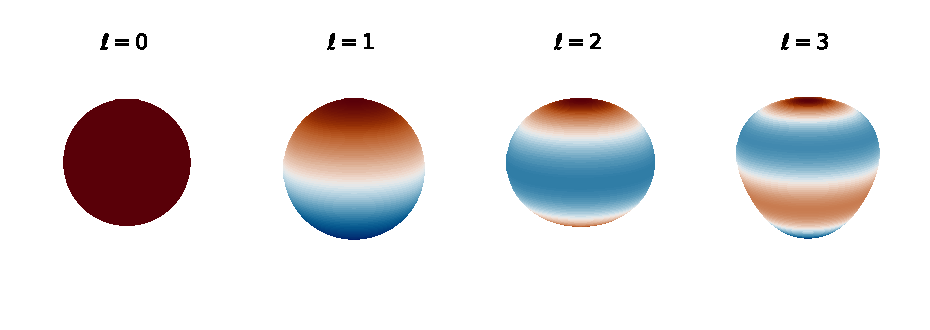
\includegraphics[trim={0 0.4in 0 0},clip]{figures/spherical_harmonics.pdf}
    \caption{Spherical harmonic oscillation modes for a few angular degrees ($l$) with azimuthal order \(m=0\). The colour-map represents the radial displacement at the surface, with \emph{red} and \emph{blue} corresponding to displacement inward and outward respectively. These regions oscillate in and out, with the white regions representing stationary nodes on the surface.}
    \label{fig:spherical-harmonics}
\end{figure}

Oscillations on the surface of a star can be approximated by spherical harmonic functions with angular degree \(l\) and azimuthal order \(m\). The angular degree is the number of nodes on the surface of the star. We show a representation of the surface spherical harmonics for the first four angular degrees in Figure \ref{fig:spherical-harmonics}. For each \(l\), there exists \(2l+1\) solutions with different azimuthal order (\(m\)) corresponding to the different orientations of the nodes over the spherical shell. Additionally, the oscillation modes have unique frequency solutions for different radial orders (\(n\)), proportional to the number of wave nodes moving radially through the star.

\begin{figure}[tb]
    \centering
    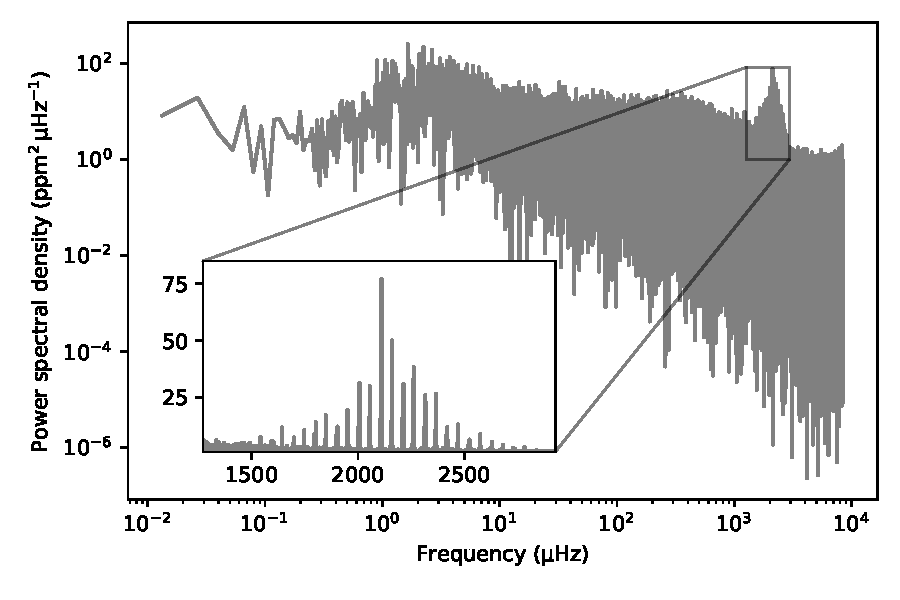
\includegraphics{figures/seismo-psd.pdf}
    \caption{The power spectral density of 16 Cyg A. The inset plot highlights the Gaussian-like power excess in the larger plot.}
    \label{fig:seismo-psd}
\end{figure}

In solar-like oscillators, p modes are stochastically excited by near-surface convection. Typically, the timescale of this process drives high-order modes (\(n \sim 20\)). We can identify these modes in a frequency-power spectrum derived from photometric or radial velocity time series observations. For instance, both stars in the 16 Cyg system are solar-like oscillators with similar properties to the Sun \needcite. Using 16 Cyg A as an example, we downloaded the power spectrum determined by the \emph{Kepler} Asteroseismic Science Operations Centre (KASOC) using \emph{Kepler} observations\footnote{\url{https://kasoc.phys.au.dk}}. Shown in Figure \ref{fig:seismo-psd}, the power spectrum of 16 Cyg A has a distinct power excess around \SI{2000}{\micro\hertz}. 

We call the location of the peak in power excess the frequency at maximum power, \(\numax\). Proportional to near-surface conditions, \citet{Brown.Gilliland.ea1991} suggested \(\numax\) scales with the acoustic cut-off frequency --- the highest frequency at which acoustic waves can reflect near the stellar surface. Hence, \citet{Kjeldsen.Bedding1995} found that \(\numax \propto g\teff^{\,-1/2}\) where \(g\) and \(\teff\) are the near-surface gravitational field strength and temperature. The power excess has a Gaussian-like shape around \(\numax\). We expect this shape to come from the distribution in convection timescale near the surface responsible for mode excitation.

Looking closely at the power excess in Figure \ref{fig:seismo-psd}, we can see a comb of approximately equally spaced peaks. Each peak corresponds to one or more oscillation modes, with its central frequency and shape providing information about the internal stellar structure. Naturally, higher frequency modes correspond to higher \(n\). However, the angular degree and azimuthal order of the modes are harder to identify. We saw in Figure \ref{fig:spherical-harmonics} how modes of higher \(l\) have more anti-nodes on the surface. Therefore, the overall effect of the oscillations cancel out when integrating over the observed surface. Consequentially, observed mode amplitude decreases with \(l\) when observing total stellar irradiance, leaving only \(l \lesssim 3\) detectable \needcite. With this assumption, we can assume the tallest peaks are \(l=0,1\) and the smaller are \(l=2,3\), modulated by the wider Gaussian-like envelope.

As an aside, the observed mode frequencies split for different \(m\) via the Doppler effect in the case of a rotating star. Measuring this splitting can constrain the rotation rate of the star. This has lead to breakthrough studies into gyrochronology and... \citep[e.g.][]{Hall.Davies.ea2021}. However, we will hereafter consider the case of a slowly rotating, spherically symmetric star, such that solutions of different \(m\) are approximately the same frequency.

If we consider an acoustic wave in a one-dimensional homogeneous medium, then we would expect each mode of oscillation to be an integer multiple of the fundamental mode. While the case for a star is more complicated, we can also approximate the frequencies for different modes as a multiple of some characteristic frequency. \citet{Tassoul1980} found that the mode frequencies could be approximated by assuming the asymptotic limit where \(l/n \rightarrow 0\), giving the following following expression \citep{Gough1986},
%
\begin{equation}
    \nu_{nl} \simeq \left(n + \frac{l}{2} + \varepsilon\right) \nu_0 + O(\nu_{nl}^{-1}), \label{eq:asy}
\end{equation}
%
where \(\varepsilon\) is some constant offset and \(O\) represents higher order terms. The characteristic frequency, \(\nu_0\), is the inverse of the acoustic diameter,
%
\begin{equation}
    \nu_0 = \left(2 \int_{0}^{R} \frac{\dd r}{c(r)}\right)^{-1},
\end{equation}
%
where \(c(r)\) is the sound speed as a function of radius, \(r\), and \(R\) is the stellar radius. \citet{Ulrich1986} found that similarly to other variable stars, this characteristic frequency relates to the mean density by \(\nu_0 \propto \overline{\rho}^{\,1/2}\). While \(\nu_0\) is not directly detectable in solar-like oscillators, we can approximate it by taking the difference between consecutive modes of the same angular degree, \(\Delta\nu_{nl} = \nu_{nl} - \nu_{n-1\,l}\). Estimates of a global (or average) large frequency separation, \(\Delta\nu \simeq \nu_0\), can thus provide information about the density of a star, leading to improved constraint on its mass and radius.

\begin{figure}[tb]
    \centering
    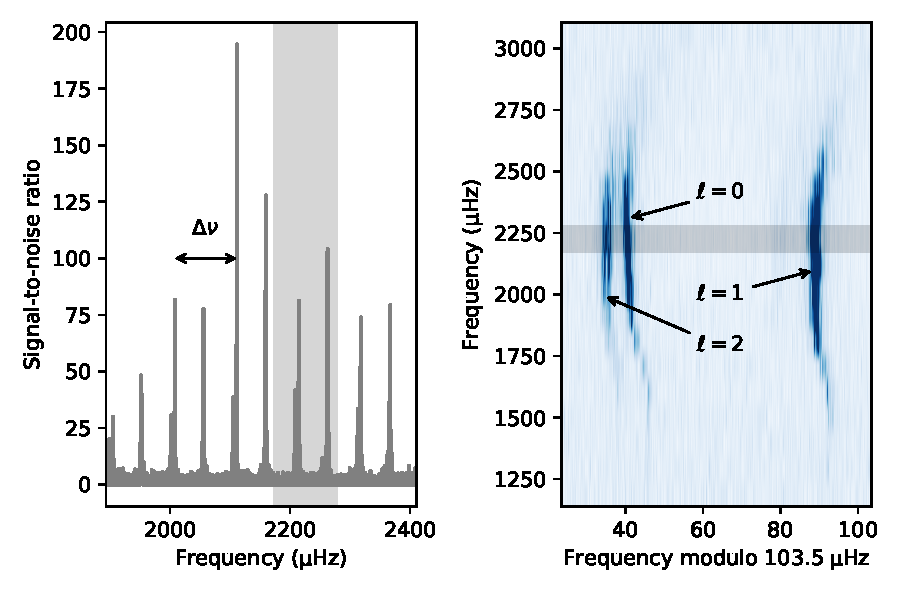
\includegraphics{figures/seismo-echelle.pdf}
    \caption{\emph{Left:} A section of the spectral signal-to-noise ratio (SNR) against frequency for 16 Cyg A. The large frequency spacing (\(\Delta\nu\)) between two radial modes is annotated with a double-headed arrow. The shaded region corresponds to a single row (also highlighted) in the echelle plot (\emph{right}). The echelle plot shows the spectral SNR such that a darker colour represents a higher SNR. Each row spans \SI{103.5}{\micro\hertz} and is stacked in order of frequency. The apparent ridges are labelled according to the angular degree (\(l\)) of the modes they represent.}
    \label{fig:seismo-echelle}
\end{figure}

The asymptotic expression helps us identify modes in a star. If Equation \ref{eq:asy} was exact, we would expect odd and even modes to be grouped together and separated by \(\dnu/2\). To see this, we revisit the power spectrum of 16 Cyg A, now with an estimate of the noise divided out. We can see the regular pattern predicted by Equation \ref{eq:asy} in the left panel of Figure \ref{fig:seismo-echelle}. Every other mode is approximately separated by \(\dnu\). To see this effect over the wider spectrum, we created an \emph{echelle} plot in the right panel. Folding the spectrum by an estimate of \(\dnu\) reveals a sequence of ridges corresponding to modes of different angular degree. Odd and even angular degree are grouped together, although do not lie on top of each other. The small difference between modes of different \(l\) is described by the higher order terms neglected from Equation \ref{eq:asy}.

% Once we have identified a solar-like oscillator, what information is there to gain from asteroseismology? We have discussed how parameters \(\numax\) and \(\dnu\) scale with global stellar properties. Scaling these parameters with respect to the Sun, we can obtain relations for the radius and mass of the star,
% %
% \begin{align}
%     \left(\frac{R}{\si{\solarradius}}\right) &\simeq \left(\frac{\numax}{\numax_{,\odot}}\right) \left(\frac{\dnu}{\dnu_\odot}\right)^{-2} \left(\frac{\teff}{\teff_{,\odot}}\right)^{1/2},\\
%     \left(\frac{M}{\si{\solarmass}}\right) &\simeq \left(\frac{\numax}{\numax_{,\odot}}\right)^3 \left(\frac{\dnu}{\dnu_\odot}\right)^{-4} \left(\frac{\teff}{\teff_{,\odot}}\right)^{3/2}.
% \end{align}
% %
% Using these relations directly can provide quick-look, independent mass and radius estimates \citep[e.g.][]{Pinsonneault.Elsworth.ea2018}.

% We can also use individual modes and compare with models. Worth noting the surface term here.


